\chapter{数值计算}
\label{ch:numerical}

\gls*{ml}算法通常需要大量的数值计算。这通常指那些解决数学问题的算法,这样的算法使
用的方法是通过一个迭代的过程,而不是给定一个对正确解的象征性的表达式分析导出一个
公式。常见的操作包括优化(找到一个参数的值,最小化或者最大化一个函数)和解线性方
程组。当函数涉及到实数,在一个计算机上即使只是对一个数学函数求值都是困难的,它无
法用有限内存精确表示。

\section{溢出和下溢}
\label{sec:overflow_and_underflow}

在一个数字计算机上做连续的数学计算的主要困难,是我们需要用一个有限的、以 bit 位的
模式的数字来表示无限多的实数。这意味着对于几乎所有的实数,当我们在计算机中表示这
些数字时引起了一些近似误差。在多数情况下,这仅仅是舍入误差。舍入误差是有问题的,
尤其是当它经过许多操作后进一步恶化,并且,如果算法没有被设计为最小化舍入误差的累
加,它们能使理论上可行的算法在实际中失败。

一种特别严重的舍入误差的形式是\emph{\gls{underflow}}。\gls*{underflow}发生在当数
字接近 $0$ 而被舍入为 $0$ 的时候。许多函数当它们的参数为 $0$ 而不是一个小的正数时
表现出本质上的不同。例如,我们通常想要避免被 $0$ 除(当这种情况发生时有些软件环境
会产生异常,其它的会返回结果为一个占位符 \verb!not-a-number! 的值)或者取 $0$ 的
对数(这通常被当作 $-\infty$ 对待,如果它被用于更进一步的算数操作会变
成 \verb!not-a-number!)。

另一个有高度破坏性的数值误差的形式是\emph{\gls{overflow}}。\gls*{overflow}发生在
当具有大的数量级的数字被近似为 $\infty$ 或 $-\infty$ 的时候。进一步的算数计算通常
把这些无限值改为 \verb!not-a-number! 值。

一个函数必须针对\gls*{underflow}和\gls*{overflow}稳定化的函数是\gls*{softmax}函
数。\gls*{softmax}函数常常被用于预测和一个多项分布关联的概率。\gls*{softmax}函数
被定义为
\begin{equation}
  \mathrm{softmax}(\pmb{x})_i = \frac{\exp(x_i)}{\sum_{j=1}^n\exp(x_j)}
\end{equation}

考虑当所有的 $x_i$ 等于某个常数 $c$ 时会发生什么。通过分析,我们能够看到所有的输
出应该等于 $\frac{1}{n}$。从数字上看,当 $c$ 有很大的数量级时这可能不会发生。如
果 $c$ 是很小的负数,那么 $\exp(c)$ 会\gls*{underflow}。这意味着\gls*{softmax}的
分母会变成 $0$,所以最后的结果是未定义的。当 $c$ 是非常大的正
数,$\exp(c)$ 会\gls*{overflow},再一次导致整个表达式为未定义的。这两个困难都能够
通过对 $\mathrm{softmax}(\pmb{z})$ ~——~这里 $\pmb{z} = \pmb{x} - \max_ix_i$
~——~求值来解决。通过分析,简单的代数显示,将输入\gls*{vec}加上或者减去一个标
量,$\mathrm{softmax}$ 函数的值不会被改变。对 $\max_ix_i$ 做减法导致 $\exp$ 有最
大的参数而为 $0$,这排除了\gls*{overflow}的可能。同样地,分母中至少一项值为 $1$,
这排除了分母中导致被 $0$ 除的\gls*{underflow}的可能。

还有一个小问题。分子上的\gls*{underflow}仍然能引起整个表达式求值为 $0$。这意味着
如果我们通过先运行 $\mathrm{softmax}$ 子程序然后传递其结果给 $\log$ 函数来实
现 $\log\mathrm{softmax(\pmb{x})}$ 时,我们会错误地得到
$-\infty$。相反,我们必需实现一个单独的函数,它以一个在数值上稳定的方式计
算 $\log\mathrm{softmax}$。$\log\mathrm{softmax}$ 函数能够使用我们用于稳定
化 $\mathrm{softmax}$ 函数的相同技巧来被稳定。

在这本书中,对于大部分内容,我们没有明确地详细说明所有涉及到实现不同算法的数值上
的考虑。底层库的开发者应该在实现\gls*{dl}算法时把数值问题记在心里。本书的大部分读
者可以简单地依赖已经提供稳定实现的底层库。在有些情况下,有可能实现一个新的算法并
且自动让新的实现稳定化。Theano
\citep{bergstra+al:2010-scipy-small,Bastien-2012}是一个软件包的例子,它自动检测并
稳定化许多常见的、出现在\gls*{dl}环境中的、数值上不稳定的表达式。

\section{不合理的条件作用}
\label{sec:poor_conditioning}

条件作用是指一个函数如何随着它的输入中的微小变化快速改变。那些当它们的输入被微小
扰动时快速变化的函数可能对科学计算是有问题的,这是因为在输入中的舍入误差可以导致
输出上的巨大变化。

考虑函数 $f(\pmb{x}) = \pmb{A}^{-1}\pmb{x}$。当 $\pmb{A} \in \mathbb{R}^{n
  \times n}$ 有一个\gls*{eigen-val}分解,它的\emph{\gls{cond-num}}\,是
\begin{equation}
  \max_{i,j}|\frac{\lambda_i}{\lambda_j}|
\end{equation}

这是最大和最小幅度的\gls*{eigen-val}的比率。当这个数很大时,矩阵求逆对于输入中的
误差是特别敏感的。

这个敏感性是矩阵本身的一个本质特性,不是在矩阵求逆中舍入误差的结果。当我们用真的
逆矩阵相乘时,条件不合理的矩阵放大了预先存在的误差。在实践中,这个误差会被求逆过
程自身中的误差进一步加剧。

\section{基于梯度的最优化}
\label{sec:gradient-based_optimization}

大部分\gls*{dl}算法涉及到某种优化。优化是指通过改变 $\pmb{x}$ 来最小化或者最大化
某个函数 $f(\pmb{x})$ 的任务。我们通常以最小化 $f(\pmb{x})$ 的形式表达大部分优化
问题。最大化可以通过一个最小化 $-f(\pmb{x})$ 的算法来完成。

我们想要最小化或者最大化的函数被称
为\emph{\gls{obj-func}}\,或者\emph{\gls{criterion}}。当我们正在最小化它的时候,我
们也可能称它\emph{\gls{cost-func}},\emph{\gls{loss-func}},或
者\emph{\gls{err-func}}。尽管有些\gls*{ml}出版物给这些术语指定特别的意义,在这本
数中,我们交换使用这些术语。

我们常常用一个上标 $*$ 表示最小化或者最大化一个函数的值。例如,我们可能
说 $\pmb{x}^* = \arg\min f(\pmb{x})$。

我们假设读者已经熟悉微积分,但是这里提供了一个关于微积分概念如何和最优化相联系的
简要回顾。

假设我们有一个函数 $y = f(x)$,其中 $x$ 和 $y$ 都是实数。这个函数的导数被表示
为 $f'(x)$ 或者 $\frac{dy}{dx}$。导数 $f'(x)$ 给出了 $f(x)$ 在点 $x$ 的斜率。换句
话说,它指定了如何调整输入中的一个小的变化,以至于获得相应的输出中的变化:$f(x +
\epsilon) \approx f(x) + \epsilon f'(x)$。

\begin{figure}[h]
  \centering
  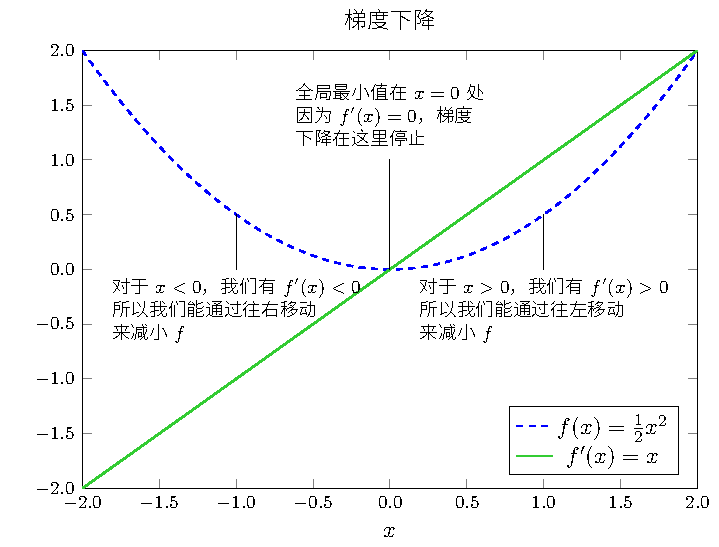
\includegraphics{gradient_descent}
  \caption{一个图例,演示一个函数的导数如何能够被用于沿着函数往下移动到一个最小值。
    这个技术被称为\emph{\gls{gradient-descent}}。\label{fig:gradient_descent}}
\end{figure}

导数对于最小化一个函数是非常有用的,因为它告诉我们如何改变 $x$ 以至于在 $y$ 上产
生一个小的改进。例如,我们知道对于足够小的 $\epsilon$,$f(x - \epsilon
\mathrm{sign}(f'(x)))$ 比 $f(x)$ 小。这样我们能够通过以导数的相反符号小步地移
动 $x$ 来减小
$f(x)$。这个技术被称为\emph{\gls{gradient-descent}}。这个技术的示例参见
图~\ref{fig:gradient_descent}。

当 $f'(x) = 0$ 时,导数没有提供关于往哪个方向移动的信息。在 $f'(x) = 0$ 的点被称
为\emph{\gls{critical-points}}\,或者\emph{\gls{stationary-points}}。一
个\emph{\gls{local-min}}\,是一个在 $f(x)$ 比所有相邻点都小的位置处的点,所以不再
可能通过做极小的步进来减小 $f(x)$。一个\emph{\gls{local-max}}\,是一个在 $(fx)$ 比
所有相邻点都大的位置处的点,所以不再可能通过做极小的步进来增加
$f(x)$。某些\gls*{critical-points}既不是最大值也不是最小值。它们被称
为\emph{\gls{saddle-points}}。每种类型的临界点参见图~\ref{fig:critical_points}。

\begin{figure}[h]
  \centering
  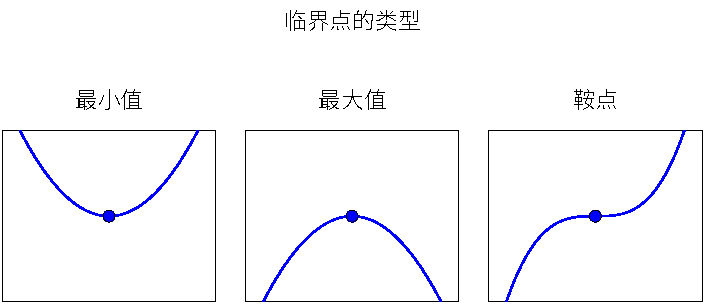
\includegraphics{critical_points}
  \caption{一维空间中三种临界点的示例。一个临界点是斜率为 $0$ 的点。这样的一个点
    既可以是一个局部最小值~——~它比相邻点更低,一个局部最大值~——~它比相邻点更高,
    也可以是一个鞍点~——~它有高于和低于这个点自身的相邻
    点。\label{fig:critical_points}}
\end{figure}

一个取得 $f(x)$ 的绝对最低值的点是一个\emph{\gls{global-min}}。函数可能存在只有一
个\gls*{global-min}或者多个\gls*{global-min}。也有可能存在并不是全局最优化的局部
最小值。在\gls*{dl}环境中,我们优化的函数可能有许多不是最优的局部最小值,而且许多
鞍点被非常平整的区域包围。所有这些使得最优化非常困难,尤其当函数的输入是多维的时
候。所以我们通常满足于找到一个非常低的 $f$ 的值,但不是必须在任何正式意义上是最小
的。参见图~\ref{fig:approximate_minimization} 的示例。

\begin{figure}[h]
  \centering
  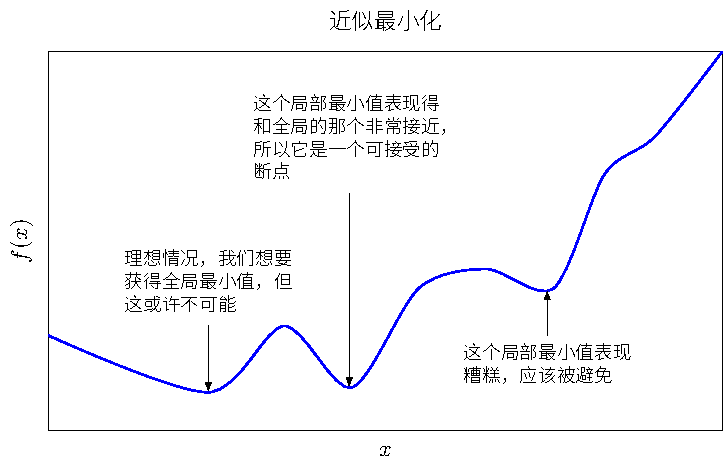
\includegraphics{approximate_minimization}
  \caption{最优化算法可能失败\label{fig:approximate_minimization}}
\end{figure}

我们常常最小化有多个输入的函数:$f: \mathbb{R}^n \rightarrow \mathbb{R}$。为了
让``最小化''的概念有意义,必须只有一个(标量)输出。

对于具有多个输入的函数,我们必须利用\emph{\gls{partial-derivatives}}\,的概念。偏
导数 $\frac{\partial}{\partial x_i}f(\pmb{x})$ 测量 $f$ 在点 $\pmb{x}$ 仅当变
量 $x_i$ 增加时如何改变。\emph{\gls{gradient}}\,概括了在导数是相对于一
个\gls*{vec}的情况下导数的概念:$f$ 的梯度是包含所有偏导数的\gls*{vec},表示
为 $\nabla_{\pmb{x}}f(\pmb{x})$。梯度中的元素 $i$ 是 $f$ 对于 $x_i$ 的偏导数。在
多维中,临界点是那些梯度中的每个元素等于 $0$ 的点。

$\pmb{u}$ 方向(一个单位\gls*{vec})上的\emph{\gls{directional-derivative}}\,是函
数 $f$ 在 $u$ 方向上的斜率。换句话说,方向导数是函数 $f(\pmb{x} +
\alpha\pmb{u})$ 对于 $\alpha$ 的导数,在 $\alpha = 0$ 处求值。使用这个链式规则,
我们能够看到
$\frac{\partial}{\partial\alpha}f(\pmb{x} + \alpha\pmb{u}) =
\pmb{u}^{\top}\nabla_{\pmb{x}}f(\pmb{x})$。

为了最小化 $f$,我们想要找到 $f$ 减小最快的方向。我们能够使用方向导数来这样做:
\begin{gather}
  \min_{\pmb{u},\pmb{u}^{\top}\pmb{u}=1}\pmb{u}^{\top}\nabla_{\pmb{x}}f(\pmb{x})\\
  = \min_{\pmb{u},\pmb{u}^{\top}\pmb{u}=1}\|\pmb{u}\|_2\|\nabla_{\pmb{x}}f(\pmb{x})\|_2\cos\theta
\end{gather}
其中 $\theta$ 是 $\pmb{u}$ 和梯度的夹角。代入 $\|\pmb{u}\|_2 = 1$ 并且忽略不依赖
于 $\pmb{u}$ 的因子,这简化为 $\min_{\pmb{u}}\cos\theta$。当 $\pmb{u}$ 指向梯度的
相反方向时其被最小化。换句话说,梯度直接指向上面,而负的梯度直接指向下面。我们能
够通过沿着负的梯度方向移动来减小
$f$。这被称为\emph{\gls{steepest-descent}}\,或者\emph{\gls{gradient-descent}}。

最陡下降提出了一个新的点
\begin{equation}
  \pmb{x}' = \pmb{x} - \epsilon\nabla_{\pmb{x}}f(\pmb{x})
\end{equation}
其中 $\epsilon$ 是\emph{\gls{learning-rate}},一个决定步长的正的标量。我们可以用
几个不同方法来选择 $\epsilon$。一个流行的方法是把 $\epsilon$ 设为一个小的常数。
有时候,我们能够解步长大小,使方向导数消失。另一种方法是对几个 $\epsilon$ 的值求
得$f(\pmb{x} - \epsilon\nabla_{\pmb{x}}f(\pmb{x}))$,选择导致最小\gls*{obj-func}
值的那个。最后一个策略被称为一个\emph{\gls{line-search}}。

最陡下降在梯度中的每个元素为 $0$ (或者,在实践中,非常接近于 $0$)时会于一点。在
某些情况下,我们可能避免运行这个迭代算法,而只是通过解 $\pmb{x}$ 的方
程 $\nabla_{\pmb{x}}f(\pmb{x}) = 0$ 直接跳到临界点。

尽管梯度下降被限制于连续空间的最优化,朝更好的配置做小的移动(即大致是最好的小的
移动)的一般概念可以推广到离散空间。上升一个离散参数的\gls*{obj-func}被称
为\emph{\gls{hill-climbing}} \citep{Russel+Norvig-book2003}。

\subsection{超越梯度:雅可比和海森矩阵}
\label{subsec:beyong_the_gradient}

有时候我们需要找到一个函数的所有偏导数,它的输入和输出都是\gls*{vecs}。包含所有这
样偏导数的矩阵被称为一个\emph{\gls{jacobian-matrix}}。具体来说,如果我们有一个函
数 $\pmb{f}: \mathbb{R}^m \rightarrow \mathbb{R}^n$,那
么 $\pmb{f}$ 的\gls*{jacobian-matrix} $\pmb{J} \in \mathbb{R}^{n \times m}$ 被定
义为 $J_{i,j} = \frac{\partial}{\partial x_j}f(\pmb{x})_i$。

有时候我们也对导数的导数感兴趣。这被称为一个\emph{\gls{second-derivative}}。例如,
对于一个函数 $f: \mathbb{R}^n \rightarrow \mathbb{R}$,$f$ 对于 $x_j$ 的导数,其
对于 $x_i$ 的导数表示为 $\frac{\partial^2}{\partial x_i \partial x_j}f$。在单个维
度中,我们能够用 $f''(x)$
表示$\frac{d^2}{dx^2}$。二阶导数告诉我们当改变输入时一阶导数会如何改变。这很重要,
因为它告诉我们一个梯度的步进是否会引起足够多的、我们期望的基于梯度自身的改进。我
们可以把二阶导数看做测量\emph{\gls{curvature}}。假设我们有一个二次函数(许多实际
出现的函数不是二次的,但是至少局部上能够被很好近似为二次)。如果这样一个函数有一
个 $0$ 的二阶导数,那么就没有曲率。它是一个完全平整的直线,而且它的值能够只使用梯
度来预测。如果梯度为 $1$,那么我们能做出一个沿着负的梯度、大小为 $\epsilon$ 的步
进,而代价函数会减少 $\epsilon$。如果二阶导数是负的,函数曲线朝下,所以代价函数实
际上会减小超过 $\epsilon$。最后,如果二阶导数是正的,函数曲线朝上,所以代价函数能
减少小于 $\epsilon$。参见图~\ref{fig:second_derivative} 来了解曲率的不同形式如何
影响通过梯度预测的代价函数的值和真实值的联系。

\begin{figure}[h]
  \centering
  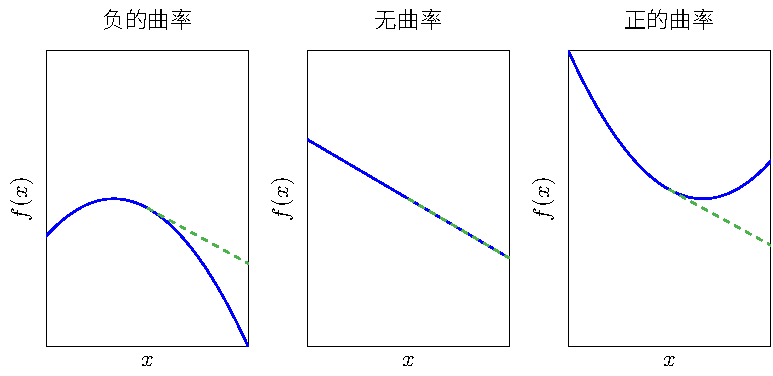
\includegraphics{second_derivative}
  \caption{二阶导数决定了一个函数的曲率。这里我们展示具有不同曲率的二次函数。虚线
    指示了代价函数的值~——~我们期望的、当做一个向下的梯度步进时只基于梯度信息的值。
    在负曲率的情况下,代价函数实际上减小得比梯度预测的更快。在无曲率的情况下,梯
    度正确预测其减小。在正曲率的情况下,函数减小得比期望的更慢,并最终开始增加,
    所以太大的步进实际上会不经意地增加函数。\label{fig:second_derivative}}
\end{figure}

当函数有多个输入维度,就有许多二阶导数。这些导数能够被收集进一个矩阵,被称
为\emph{\gls{hessian-matrix}}。\gls*{hessian-matrix} $\pmb{H}(f)(\pmb{x})$ 被定义
为这样
\begin{equation}
  \pmb{H}(f)(\pmb{x})_{i,j} = \frac{\partial^2}{\partial x_i \partial x_j}f(\pmb{x})
\end{equation}
相等地,海森矩阵是梯度的雅可比矩阵。

任何二阶偏导数连续的地方,微分算子满足交换律,即,它们的顺序可交换:
\begin{equation}
  \frac{\partial^2}{\partial x_i \partial y_j}f(\pmb{x}) = \frac{\partial^2}{\partial x_j \partial x_i}f(\pmb{x})
\end{equation}
这意味着
$H_{i,j} = H_{j,i}$,所以\gls*{hessian-matrix}在这样的点是对称的。我们
在\gls*{dl}环境中碰到的大部分函数有一个几乎在任何位置对称的\gls*{hessian-matrix}。
因为\gls*{hessian-matrix}是实数矩阵并且是对称的,我们能够把它分解成一个实
数\gls*{eigen-vals}集合和一个\gls*{eigen-vecs}的正交基。在一个由一个单
位\gls*{vec} $\pmb{d}$ 表示的特定方向上的二阶导数,
由 $\pmb{d}^{\top}\pmb{H}\pmb{d}$ 得出。当 $\pmb{d}$ 是 $\pmb{H}$ 的一
个\gls*{eigen-vec},那个方向上的二阶导数由相应的\gls*{eigen-val}得出。对于其
它 $\pmb{d}$ 的方向,方向性的二阶导数是所有\gls*{eigen-vals}的一个加权平均,具
有 $0$ 和 $1$ 之间的权重,并且和 $\pmb{d}$ 有更小夹角的\gls*{eigen-vecs}接收更多
权重。最大的\gls*{eigen-val}决定了最大的二阶导数,而最小的\gls*{eigen-val}决定了
最小的二阶导数。

(方向性的)二阶导数告诉我们能期待一个梯度下降的步进表现得怎样好。我们可以做一个
二阶泰勒级数,在当前点 $\pmb{x}^{(0)}$ 处逼近函数 $f(\pmb{x})$:
\begin{equation}
  f(\pmb{x}) \approx f(\pmb{x}^{(0)}) + (\pmb{x} - \pmb{x}^{(0)})^{\top}\pmb{g} + \frac{1}{2}(\pmb{x} - \pmb{x}^{(0)})^{\top}\pmb{H}(\pmb{x} - \pmb{x}^{(0)})
\end{equation}
这里 $\pmb{g}$ 是梯度,$\pmb{H}$ 是在点 $\pmb{x}^{(0)}$ 的\gls*{hessian-matrix}。
如果我们使用一个 $\epsilon$ 的\gls*{learning-rate},那么新的
点 $\pmb{x}$ 会由 $\pmb{x}^{(0)} - \epsilon\pmb{g}$ 得出。把这代入我们的近似方程,
我们得到
\begin{equation}
  f(\pmb{x}^{(0)} - \epsilon\pmb{g}) \approx f(\pmb{x}^{(0)}) - \epsilon\pmb{g}^{\top}\pmb{g} + \frac{1}{2}\epsilon^2\pmb{g}^{\top}\pmb{H}\pmb{g}
\end{equation}
这里有三个项:函数的原始值,由函数斜率引起的期望的改进,以及为了把函数曲率计算在
内我们必需应用的校正。当最后一项非常大时,梯度下降步进实际上能够往上移动。当
$\pmb{g}^{\top}\pmb{H}\pmb{g}$ 是 $0$ 或负数,泰勒级数近似预测了不断地增加
$\epsilon$ 会不断地减小 $f$。在实践中,对于大的 $\epsilon$ 泰勒级数不太可能保持
准确,所以在这种情况下必需借助于更有启发式的 $\epsilon$ 的选择。当
$\pmb{g}^{\top}\pmb{H}\pmb{g}$ 是正的,求解最优的步长~——~最大地减小函数的泰勒级
数近似~——~得出
\begin{equation}
  \epsilon^* = \frac{\pmb{g}^{\top}\pmb{g}}{\pmb{g}^{\top}\pmb{H}\pmb{g}}
\end{equation}

在最坏的情况下,当 $\pmb{g}$ 和 $\pmb{H}$ 对应于最大\gls*{eigen-val}
$\lambda_{\max}$ 的\gls*{eigen-vec}对齐,那么这个最优步长由
$\frac{1}{\lambda_{\max}}$ 得出。为了达到我们最小化的函数能够很好地被一个二次函
数近似的程度,于是\gls*{hessian-matrix}的\gls*{eigen-vals}确定了
\gls*{learning-rate}的大小。

二阶导数可以被用于确定一个临界点是否是一个局部最大值、局部最小值,或者鞍点。回想
到在一个临界点上,$f'(x) = 0$。当 $f''(x) > 0$,这意味着当我们往右移动
时 $f'(x)$增加,当往左移动时 $f'(x)$ 减小。这意味着对于足够小
的 $\epsilon$,$f'(x - \epsilon) < 0$
而$f'(x + \epsilon) > 0$。换句话说,当我们往右移动,斜率开始指向右上方,而当我们
往左移动,斜率开始指向左上方。这样,当 $f'(x) = 0$ 而 $f''(x) > 0$ 时,我们能得出
结论 $x$ 是一个局部最小值。相似地,当 $f'(x) = 0$ 而 $f''(x) < 0$ 时,我们能得出
结论 $x$ 是一个局部最大值。这被称为\emph{\gls{second-derivative-test}}。不幸的是,
当 $f''(x) = 0$,检测是不确定的。在这种情况下,$x$ 可能是一个鞍点,或者是一个平整
区域的一部分。

在多个维度中,我们需要检查函数的所有二阶导数。使用\gls*{hessian-matrix}的特征分解,
我们能够把\gls*{second-derivative-test}概括为多个维度。在一个临界
点,$\nabla_{\pmb{x}}f(\pmb{x}) = 0$,我们能够检
查\gls*{hessian-matrix}的\gls*{eigen-vals}来确定临界点是否是一个局部最大值、局部
最小值或鞍点。当\gls*{hessian-matrix}是正无穷(它的所有\gls*{eigen-vals}是正的),
这个点是一个局部最小值。这可以通过观察在任意方向上的方向性的二阶导数来理解,并参
考单变量的\gls*{second-derivative-test}。同样的,当\gls*{hessian-matrix}是负无穷
(它的所有\gls*{eigen-vals}是负的),这个点是一个局部最大值。在多个维度中,有些情
况下实际上有可能找到鞍点的正的迹象。当至少一个\gls*{eigen-val}是正的以及至少一
个\gls*{eigen-val}是负的时候,我们知道 $\pmb{x}$ 在一个 $f$ 的横截面上是一个局部
最大值,但是在另一个横截面上是一个局部最小值。参见图~\ref{fig:saddle_point} 的示
例。最后,正如单变量的版本,多维的\gls*{second-derivative-test}可以是不确定的。无
论当所有的非零\gls*{eigen-vals}有相同符号,但至少一个\gls*{eigen-val}是 $0$ 的时
候,检测是不确定的。这是因为单变量的\gls*{second-derivative-test}在对应于
零\gls*{eigen-val}的横截面上是不确定的。

\begin{figure}[h]
  \centering
  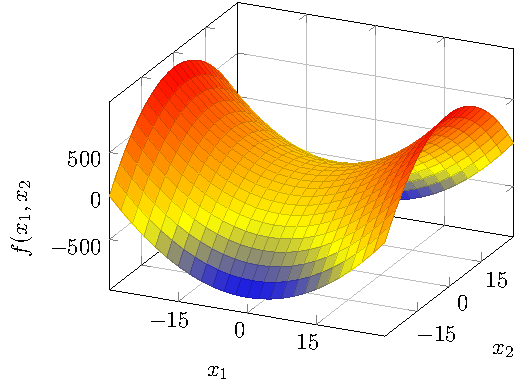
\includegraphics{saddle_point}
  \caption{一个包含正和负曲率的鞍点。这个函数示例是 $f(\pmb{x}) = x^2_1 - x^2_2$。
    沿着对应于 $x_1$ 的坐标轴,函数的曲线朝上。这个坐标轴
    是\gls*{hessian-matrix}的一个\gls*{eigen-vec}并有一个正的\gls*{eigen-val}。沿
    着对应于 $x_2$ 的坐标轴,函数曲线朝下。这个方向是\gls*{hessian-matrix}的一个
    具有负的\gls*{eigen-val}的\gls*{eigen-vec}。``鞍点''这个名称衍生自这个函数的
    马鞍形状。这是一个函数有一个鞍点的典型例子。在超过一个的维度中,为了取得一个
    鞍点,并不必需要有一个为 $0$ 的\gls*{eigen-val}:唯一必需的是既有正的又有负
    的\gls*{eigen-vals}。我们能够把一个鞍点看做既是在一个横截面中的局部最大值又是
    在其它横截面中的局部最小值的\gls*{eigen-vals}的符
    号。\label{fig:saddle_point}}
\end{figure}

在多个维度中,因为在每个方向上有不同的二阶导数,在单个点上能够有很多不同的二阶导
数。\gls*{hessian-matrix}的条件数衡量二阶导数的变化了多少。当
\gls*{hessian-matrix}有一个很差的条件数,梯度下降表现得很差。这是因为在一个方向
上,导数增加地很快,同时在另一个方向上,它则缓慢减小。梯度下降并没有意识到导数中
的这个变化,所以它不知道它需要优先检查导数长时间里保持负值的方向。它也使得选择一
个好的步长变得困难。步长必须足够小,以避免超过最小值,并在具有较强正曲率的方向上
上升。这通常意味着在其他具有较小曲率的方向上,步长太小而不能产生显著的进展。参见
图~\ref{fig:curvature_in_hessian} 的一个例子。

\begin{figure}[h]
  \centering
  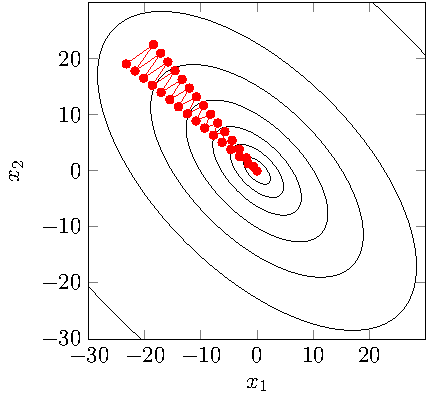
\includegraphics{curvature_in_hessian}
  \caption{梯度下降未能利用包含在\gls*{hessian-matrix}中的曲率信息。这里我们使用
    梯度下降来最小化一个二次函数 $f(\pmb{x})$,其\gls*{hessian-matrix}的条件数为
    $5$。这意味着曲率最大的方向比曲率最小的方向多 5 倍的曲率。在这例子中,最大曲
    率位于方向 ${[1,1]}^{\top}$,而最小曲率位于 ${[1,-1]}^{\top}$ 方向。红色的线
    表示梯度下降沿着的路径。这个很长的二次函数类似于一个长的峡谷。梯度下降重复地
    把时间浪费在下降峡谷的侧壁,因为他们是最陡的特征。由于步长过大,它有一个冲过
    函数底部的趋势,因此需要在下一次迭代是在对面的峡谷侧壁上下降。
    \gls*{hessian-matrix}的大的正\gls*{eigen-val}~——~对应于指向指这一方向的
    \gls*{eigen-vec}~——~表明该方向导数的急剧增加,所以一个基于
    \gls*{hessian-matrix}的优化算法可以预测最速方向实际上不是在这种环境中有用的
    搜索方向。\label{fig:curvature_in_hessian}}
\end{figure}

\section{受约束的最优化}
\label{sec:constrained_optimization}

\section{示例:线性最小二乘法}
\label{sec:example:linear_least_squares}
